\chapter{Krav}
I starten af projektet var der opstillet nogle krav til produktet. Systemet skulle være i stand til at indsamle EKG-data, detektere en selvvalgt hjertesygdom og lagre abnormale EKG-signalers data i en database. Disse krav ligger til grund for de tre væsentligste Use Cases, som det ses på figur 5.1

\begin{figure}[H]
	\centering
	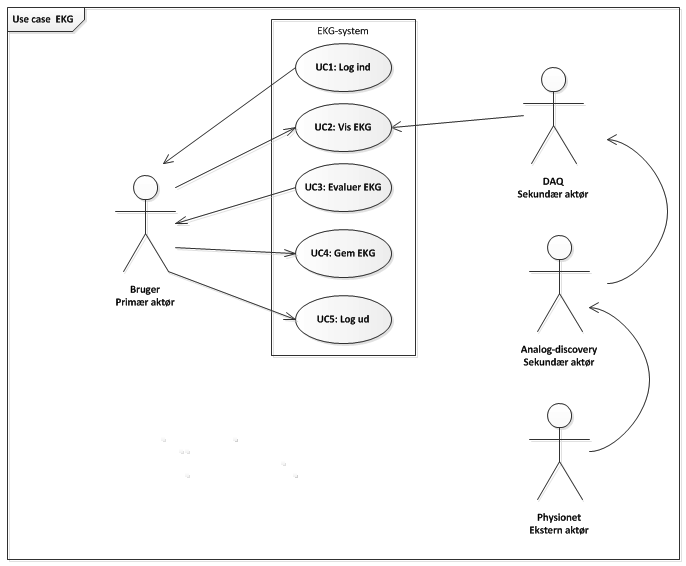
\includegraphics[width=0.8\textwidth]{Figurer/Snip20150518_11}
	\caption{Use case-diagram}
	\label{fig:Use Cases}
\end{figure}

Som vist på figuren, er der i alt 5 Use Cases som beskriver, systemets funktionelle krav. De vigtigste Use Cases er UC2, UC3 og UC4, da de udgør de i forvejen opstillede krav til projektet. Inden programmet kan startes er der dog tilføjet visse krav til anvendelse. Hver bruger skal have et personligt login, så de på den måde "underskriver" målingerne, der foretages. Det gør det nemmere at rette henvendelse i tilfælde af spørgsmål til enkelte målinger. Desuden skal patientens CPR-nummer indtastes, således at EKG-signalets data gemmes i forhold til den pågældende patient.\\
Når EKG-signalet evalueres er programmet indstillet til at detektere sygdommen atrieflimren. Hvis denne arytmi fremgår på EKG-grafen, meldes dette til brugeren af systemet. Dermed ved brugeren, at der skal holdes øje med denne sygdom.\\
Når EKG-målinger gemmes vil de blive gemt i en privat- og offentlig database. Målingerne gemmes i forbindelse med et patientId, som er koblet sammen med patientens CPR-nummer. Dermed gøres det nemmere for sundhedsfaglig personale at finde den enkelte patients målinger.\\
De ikke-funktionelle krav er beskrevet udfra (F)URPS+ og MoSCOW metoden. Her beskrives, hvilke krav der stilles til systemets interface og pålidelighed.\\
For yderligere beskrivelse af både funktionelle og ikke-funktionelle krav se dokumentation 2.2 og 2.3\\
 